\documentclass{article}[18pt]
\ProvidesPackage{format}
%Page setup
\usepackage[utf8]{inputenc}
\usepackage[margin=0.7in]{geometry}
\usepackage{parselines} 
\usepackage[english]{babel}
\usepackage{fancyhdr}
\usepackage{titlesec}
\hyphenpenalty=10000

\pagestyle{fancy}
\fancyhf{}
\rhead{Sam Robbins}
\rfoot{Page \thepage}

%Characters
\usepackage{amsmath}
\usepackage{amssymb}
\usepackage{gensymb}
\newcommand{\R}{\mathbb{R}}

%Diagrams
\usepackage{pgfplots}
\usepackage{graphicx}
\usepackage{tabularx}
\usepackage{relsize}
\pgfplotsset{width=10cm,compat=1.9}
\usepackage{float}

%Length Setting
\titlespacing\section{0pt}{14pt plus 4pt minus 2pt}{0pt plus 2pt minus 2pt}
\newlength\tindent
\setlength{\tindent}{\parindent}
\setlength{\parindent}{0pt}
\renewcommand{\indent}{\hspace*{\tindent}}

%Programming Font
\usepackage{courier}
\usepackage{listings}
\usepackage{pxfonts}

%Lists
\usepackage{enumerate}
\usepackage{enumitem}

% Networks Macro
\usepackage{tikz}


% Commands for files converted using pandoc
\providecommand{\tightlist}{%
	\setlength{\itemsep}{0pt}\setlength{\parskip}{0pt}}
\usepackage{hyperref}

% Get nice commands for floor and ceil
\usepackage{mathtools}
\DeclarePairedDelimiter{\ceil}{\lceil}{\rceil}
\DeclarePairedDelimiter{\floor}{\lfloor}{\rfloor}

% Allow itemize to go up to 20 levels deep (just change the number if you need more you madman)
\usepackage{enumitem}
\setlistdepth{20}
\renewlist{itemize}{itemize}{20}

% initially, use dots for all levels
\setlist[itemize]{label=$\cdot$}

% customize the first 3 levels
\setlist[itemize,1]{label=\textbullet}
\setlist[itemize,2]{label=--}
\setlist[itemize,3]{label=*}

% Definition and Important Stuff
% Important stuff
\usepackage[framemethod=TikZ]{mdframed}

\newcounter{theo}[section]\setcounter{theo}{0}
\renewcommand{\thetheo}{\arabic{section}.\arabic{theo}}
\newenvironment{important}[1][]{%
	\refstepcounter{theo}%
	\ifstrempty{#1}%
	{\mdfsetup{%
			frametitle={%
				\tikz[baseline=(current bounding box.east),outer sep=0pt]
				\node[anchor=east,rectangle,fill=red!50]
				{\strut Important};}}
	}%
	{\mdfsetup{%
			frametitle={%
				\tikz[baseline=(current bounding box.east),outer sep=0pt]
				\node[anchor=east,rectangle,fill=red!50]
				{\strut Important:~#1};}}%
	}%
	\mdfsetup{innertopmargin=10pt,linecolor=red!50,%
		linewidth=2pt,topline=true,%
		frametitleaboveskip=\dimexpr-\ht\strutbox\relax
	}
	\begin{mdframed}[]\relax%
		\centering
		}{\end{mdframed}}



\newcounter{lem}[section]\setcounter{lem}{0}
\renewcommand{\thelem}{\arabic{section}.\arabic{lem}}
\newenvironment{defin}[1][]{%
	\refstepcounter{lem}%
	\ifstrempty{#1}%
	{\mdfsetup{%
			frametitle={%
				\tikz[baseline=(current bounding box.east),outer sep=0pt]
				\node[anchor=east,rectangle,fill=blue!20]
				{\strut Definition};}}
	}%
	{\mdfsetup{%
			frametitle={%
				\tikz[baseline=(current bounding box.east),outer sep=0pt]
				\node[anchor=east,rectangle,fill=blue!20]
				{\strut Definition:~#1};}}%
	}%
	\mdfsetup{innertopmargin=10pt,linecolor=blue!20,%
		linewidth=2pt,topline=true,%
		frametitleaboveskip=\dimexpr-\ht\strutbox\relax
	}
	\begin{mdframed}[]\relax%
		\centering
		}{\end{mdframed}}
\lhead{Software Methodologies - Image Processing}


\begin{document}
\begin{center}
\underline{\huge Image Compression}
\end{center}
\section{Redundancy in images}
We can compress images by targeting three principal types of redundancy
\begin{definition}[Coding redundancy]
Use of sub-optimal codes means that we may use more bits than are needed to represent the pixel values
\end{definition}
\begin{definition}[Spatial redundancy]
Neighbouring pixels are likely to have similar values. Information may be unnecessarily replicated in the representation of spatially correlated pixels 
\end{definition}
\begin{definition}[Irrelevant information]
Images may contain visually non essential information that is ignored by the human visual system
\end{definition}
\section{Lossy vs Lossless Compression}
Lossy compression:
\begin{itemize}
	\item Used when images need not be reproduced exactly and an approximation is OK
	\item Compression artefacts in the image, which may not be visible
	\item Source of noise for image processing and computer vision algorithms
	\item Widely used, efficient implementations exists
\end{itemize}
Lossless compression:
\begin{itemize}
	\item Computationally more expensive
	\item Resulting file size often larger than corresponding lossy compression files
	\item No additional noise to the image
	\item Generally less widely used
\end{itemize}
\section{JPEG}
JPEG is an image compression algorithm based on the Discrete Cosine Transform and variable length encoding.\\
\\
Offers tunable (user controlled quality) lossy compression
\subsection{DCT}
The 1D DCT expresses a vector of data points, here pixel intensity values, as a weighted sum of cosine functions of varying frequencies. Essentially a variation of DFT.\\
\\
Similarly to the DFT, DCT can also be seen as a mathematical change of basis, which can be described as multiplication of the data vector by a special matrix, here the DCT matrix.\\
\\
Unlike the DFT, DCT is a real transform and not a complex one. The elements of the DCT matrix and real numbers.
\subsubsection{Basis functions}
The 2D DCT uses a set of 2D matrices as basis functions, each one corresponding to a 2D cosine function
\begin{center}
	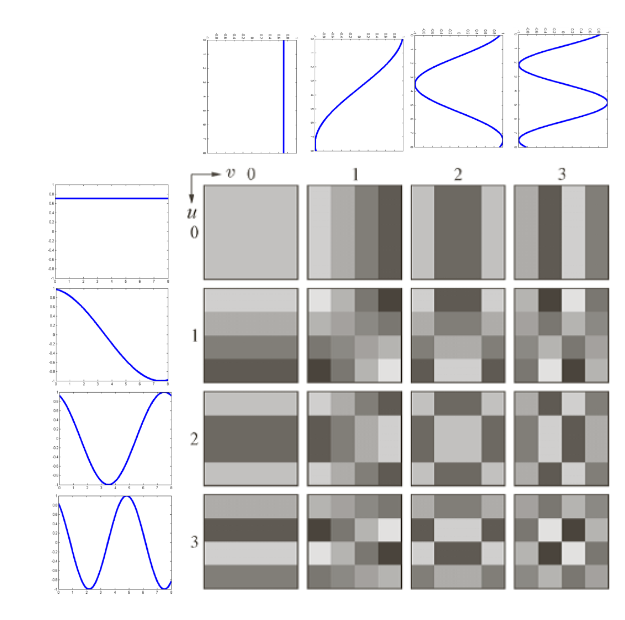
\includegraphics[scale=0.7]{Basis_Functions}
\end{center}
\subsection{JPEG Compression}
\textbf{Step 1} - Subdivide the image into pixel blocks of 8x8 size. The blocks are processed one after the other from left to right and top to bottom.\\
\\
\textbf{Step 2} - Assuming that the values of the pixels are in the range [0,255], subtract 128 to bring them into the range [-128,127]. This is done as the DCT maps that interval on itself.\\
\\
\textbf{Step 3} - Apply the 8x8 DCT to each block. The DCT values are computed with 11-bit precision (even though the input has 8-bit precision)\\
\\
\textbf{Step 4} - Scale and quantize the DCT values, using the following quantisation matrix
$$Z=\left(\begin{array}{cccccccc}
16 & 11 & 10 & 16 & 24 & 40 & 51 & 61 \\
12 & 12 & 14 & 19 & 26 & 58 & 60 & 55 \\
14 & 13 & 16 & 24 & 40 & 57 & 69 & 56 \\
14 & 17 & 22 & 29 & 51 & 87 & 80 & 62 \\
18 & 22 & 37 & 56 & 68 & 109 & 103 & 77 \\
24 & 35 & 55 & 64 & 81 & 104 & 113 & 92 \\
49 & 64 & 78 & 87 & 103 & 121 & 120 & 101 \\
72 & 92 & 95 & 98 & 112 & 100 & 103 & 99
\end{array}\right)$$
That is, if $T(u,v)$ is the DCT of the 8x8 pixel block, we do component wise division of the two matrices and round the result
$$\hat{T}(u, v)=\operatorname{round}\left[\frac{T(u, v)}{Z(u, v)}\right]$$
The quality of the image is controlled by a user parameter which determines the Z matrix\\
\\
\textbf{Step 5} - create a sequence of the quantised DCT coefficients $\hat{T}(u,v)$ using the zig zag pattern
$$\begin{array}{cccccccc}
0 & 1 & 5 & 6 & 14 & 15 & 27 & 28 \\
2 & 4 & 7 & 13 & 16 & 26 & 29 & 42 \\
3 & 8 & 12 & 17 & 25 & 30 & 41 & 43 \\
9 & 11 & 18 & 24 & 31 & 40 & 44 & 53 \\
10 & 19 & 23 & 32 & 39 & 45 & 52 & 54 \\
20 & 22 & 33 & 38 & 46 & 51 & 55 & 60 \\
21 & 34 & 37 & 47 & 50 & 56 & 59 & 61 \\
35 & 36 & 48 & 49 & 57 & 58 & 62 & 63
\end{array}$$
\textbf{Step 6} - Encode the sequence of quantised coefficients $\hat{T}(u,v)$ obtained in step 5 with a Huffman based variable length code, encoding each coefficients value and the number of preceeding zeros.\\
\\
Use a special symbol for the end of non-zero coefficients

\end{document}